\documentclass[citenumber]{llncs}
%
\usepackage{makeidx}  % allows for indexgeneration
%
\usepackage{hyperref}				% enlaces en el pdf
\hypersetup{colorlinks=true,        % colores en vez de cajas en los enlaces
			linkcolor=blue,         % color of internal links (change box color with linkbordercolor)
    		citecolor=blue,         % color of links to bibliography
    		filecolor=blue,         % color of file links
    		urlcolor=blue}          % color of external links	    

\usepackage{algorithm}
\usepackage{setspace}				% Para el seudocódigo
\usepackage{amsmath}				% Para el seudocódigo
\usepackage[noend]{algpseudocode}	% Para el seudocódigo
\usepackage{multicol}				% Para el seudocódigo
\usepackage{graphicx}           	% para manejar imagenes
\usepackage[utf8]{inputenc}

\begin{document}
\mainmatter              % start of the contributions
%
\title{MiLIT vs. MinReduct: a comparative study.}
			 
\author{Vlad\'{i}mir Rodr\'{i}guez--Diez\inst{1,2} \and Jos\'{e}~Fco. Mart\'{i}nez--Trinidad\inst{3}
		 \and J.~Ariel Carrasco--Ochoa\inst{3} \and Manuel~S.~Lazo--Cortés\inst{3} \and J. Arturo Olvera--López\inst{1}}
%
\authorrunning{Vlad\'{i}mir Rodr\'{i}guez et al.} % abbreviated author list (for running head)
%
\institute{Benemérita Universidad Autónoma de Puebla,\\
	Faculty of Computer Science,\\
	Language \& Knowledge Engineering Lab,\\
	Av. del Infante S/N, Ciudad Universitaria, Puebla, Pue. México\\
\and Universidad de Camag\"{u}ey,\\
	Circunvalaci\'{o}n Nte. km 5$\frac{1}{2}$, Camag\"{u}ey, Cuba\\
	\email{vladimir.rodriguez@reduc.edu.cu}
\and Instituto Nacional de Astrof\'{i}sica, \'{O}ptica y Electr\'{o}nica,\\
	 Luis Enrique Erro \# 1, Tonantzintla, Puebla, M\'{e}xico,\\
	 Coordinaci\'{o}n de Ciencias Computacionales,\\}


\maketitle              % typeset the title of the contribution

\begin{abstract}
	Rough set reducts are irreducible subsets of attributes preserving discernibility information of an decision system. Computing all reducts has exponential complexity regarding the number of attributes in the decision system. Given the high computational cost of this task, computing only the reducts of minimum length (the shortest reducts) becomes relevant for a wide range of applications. Two recent algorithms have been reported, almost simultaneously, for computing this irreducible subsets of attributes with minimum length: MiLIT and MinReduct. MiLIT was designed in the top of the Testor Theory while MinReduct comes from the Rough Set Theory. Both algorithms are intended to solve an equivalent algorithmic task. Thus, in this paper we present a comparative study of these algorithms in terms of asymptotic complexity and runtime performance. 
	
\keywords{Typical Testor, Reduct, minimum--length, shortest}
\end{abstract}
%
\section{Introduction}
%
	Rough Set Theory (RST)~\cite{Pawlak82} Reducts are minimal subsets of attributes preserving the discernibility capacity of the whole set of attributes \cite{Pawlak91}. Reducts have been found useful for feature selection~\cite{Nguyen2016,Alwesabi2016}, attribute relevance evaluation~\cite{Inuiguchi2017} and classification~\cite{Ishii2018,Own2015} among others. The main drawback of reducts is that computing the complete set of reducts for a decision system is an NP--hard problem~\cite{Skowron92}. However, most of the times, only a subset of reducts is sufficient for real applications~\cite{Zheng14,Jiang15}. The set of all the reducts with the minimum length (the shortest reducts) is particularly relevant for such applications, since it is a representative sample of all reducts~\cite{Susmaga1998}. Recently, the new algorithm MinReduct, for computing all the shortest reducts, was reported~\cite{rodriguez20}. Although the problem of computing all the shortest reducts of a decision system is also NP--hard, it is usually significantly faster than computing all reducts.
	
	Testor Theory~\cite{Cheguis55} separately developed the concept of Typical Testor. Typical Testor and Reduct concepts are so close~\cite{Chikalov2013}, that algorithms designed for computing typical testors can be used for computing reducts and vice versa~\cite{Lazo15}. Typical testors have been used for feature selection~\cite{Dmitriev1966,Ruiz08} and some other real--world applications~\cite{Torres2014}. Since computing all typical testors is also NP--hard, a significant runtime reduction, can be obtained from computing only the set of all the minimum--length typical testors. For this purpose, the MiLIT algorithm was recently published~\cite{Piza20}. The authors reported indeed two variants of MiLIT: the first one using an in-place search based on Next
	Combination calculation (NC) and the other one using a search with Pruning based on Feature and
	Row Contributions (PFRC).
		
	The almost simultaneous publication of these algorithms that solve an equivalent problem deserves a comparative study. Thus, in this work, we present such a study with the aim of providing application suggestions and some foundations for the development of future algorithms. To this end, we will first provide a common theoretical framework for describing the algorithms under study. Then, a description in terms of asymptotic complexity will be presented. Finally, an experimental assessment of the three algorithms will be carried out over synthetic and real--world decision systems. 
	
	% Estructura del documento
	The rest of this paper is structured in the following way. In Section~\ref{tb}, some basic concepts from RST and the theoretical basis of the pruning properties used by the algorithms under study are presented. In Section~\ref{Algs}, we describe the algorithms with an special emphasis in their asymptotic time complexity. Then, in Section~\ref{Comparison}, we present our experimental assessment and the discussion of the results. Finally, our conclusions appear in Section~\ref{conclusions}.
						
%
\section{Theoretical background} \label{tb}
%

	In this section, we introduce the main concepts of Rough Set Theory, as well as the definitions and propositions supporting the pruning strategies used in MiLIT and MinReduct. Notice that although MiLIT algorithms are designed in the top of Testor Theory, we will use concepts from Rough Set Theory for describing these algorithms.

%
\subsection{Basic Concepts} \label{basic_concetps}
%
	In RST, a decision system ($DS$) is a table with rows representing objects while columns represent attributes. We denote by $U$ a finite non-empty set of objects $U=\lbrace x_1,x_2,...,x_n\rbrace$ and $A$ is a finite non-empty set of attributes. For every attribute in $A$ there is a mapping: $a: U \rightarrow V_a$. The set $V_a$ is called the \textit{value set} of $a$. Attributes in $A$ are further divided into condition attributes $C$ and decision attributes $D$ such that $A=C \cup D$. 

	Decision attributes $D$ induce a partition of the universe $U$ into decision classes. Usually, we are interested in those classes induced by $B$ that correspond to the decision classes. To this end, the \textit{B-positive region of D}, denoted as $POS_B(D)$, is defined as the set of all objects in $U$ such that if two of them have the same value for every attribute in B, they belong to the same decision class.

	A subset $B \subseteq C$ is a decision \textit{reduct} of $DS$ relative to $D$ if
	\begin{enumerate}
		\item $POS_B(D)=POS_C(D)$. \label{cond_1}
		\item $B$ is a minimal subset (with respect to inclusion) satisfying condition~\ref{cond_1}.\label{cond_2}
	\end{enumerate}

	Decision reducts have the same capability as the complete set of condition attributes for discerning between objects from different classes (Condition~\ref{cond_1}), and every attribute in a reduct (typical testor) is indispensable for holding Condition~\ref{cond_1} (Condition~\ref{cond_2}). A super--reduct (testor) is a set $B$ that satisfies Condition~\ref{cond_1}, regardless of Condition~\ref{cond_2}. Decision reducts are called just reducts, for simplicity.

	The \textit{Binary Discernibility Matrix} is a binary table representing the discernibility information of objects belonging to different classes. The element $m(i, j, c)$ regarding two objects $x_i$ and $x_j$ and a single condition attribute $c \in C$ is defined as:

	\begin{equation*}
		m(i, j, c)=\left\lbrace\begin{array}{cl}
		1 & \mathrm{if~~}c(x_i) \neq c(x_j) \\
		0 								   & \mathrm{otherwise} 
		\end{array}\right.
	\end{equation*} 

	The \textit{Simplified Binary Discernibility Matrix} is a reduced version of the binary discernibility matrix after applying absorption laws. In Testor Theory~\cite{Lazo01} this concept is called \textit{Basic Matrix}, and we will adopt this term for the rest of this document, because it is simple and explicit. From the basic matrix of a decision system all reducts can be computed~\cite{Yao09}.

%	
\subsection{Pruning properties used by the algorithms under study}
%
	The reader can find the proof and a more detailed explanation of the following propositions in~\cite{rodriguez20,Piza20}. 
	
	\begin{definition}\label{def:testor}
		$B$ is a super--reduct iff in the sub--matrix of the basic matrix formed by the columns corresponding to the attributes in $B$, there is no zero row (a row with only zeros).
	\end{definition}
	
	The attribute contribution, presented in Definition~\ref{def:contrib}, is used by MinReduct and PFRC--MiLIT. 	
	
	\begin{definition}\label{def:contrib}
		Given $B \subseteq C$ and $x_i \in C$ such that $x_i \notin B$. $x_i$ contributes to $B$ iff the sub-matrix of the basic matrix formed with only those attributes in $B$ has more zero rows than that matrix formed with attributes in $B \cup \lbrace x_i \rbrace$.
	\end{definition}	
	
	The pruning based on Definition~\ref{def:contrib} is supported by Proposition~\ref{prop:contrib}.
	
	\begin{proposition}\label{prop:contrib} 
		Given $B \subseteq C$ and  $x_i \in C$ such that $x_i \notin B$. If $x_i$ does not contribute to $B$, then $B\cup\{x_i\}$ cannot be a subset of any reduct.
	\end{proposition}
	
	The algorithms under study search for super--reducts (testors) instead of reducts (typical testors) supported by the following proposition, which was first introduced in~\cite{Zhou2009}. This simplification reduces the cost of candidate subsets evaluations.
	
	\begin{proposition}\label{prop:sr} 
		Let $B \subseteq C$, if $B$ is one of the shortest super--reducts of a basic matrix, then it is also one of the shortest reducts.
	\end{proposition}	

	MiLIT and MinReduct, as in many other algorithms for reduct (and typical testor) computation~\cite{Sanchez07,Lias13,Rodriguez2018} arrange the basic matrix in order to reduce the search space. The arrangement consist in moving one of the rows with the fewest number of 1's in the basic matrix to the top, and all columns in which this row has 1, are moved to the left. This arrangement reduces the attributes combinations evaluated by these algorithms which follow a traversing order that resembles the lexicographical order. The search can be stopped after all the combinations that include a column with a 1 in the first row are evaluated. For the rest of the search space, the first row is always a zero row.
	
	For PFRC--MiLIT the following proposition was presented:
	
	\begin{proposition}\label{prop:zrPrevail} 
		Given $B \subseteq C$ and  $x_i \in C$ such that $x_i \notin B$. If there exist a zero row in the sub--matrix of the basic matrix formed by the attributes in $B\cup\{x_i\}$, that is also a zero row in the sub--matrix formed by the remaining attributes on the right side of $x_i$. Then $B\cup\{x_i\}$ cannot be a subset of any reduct.
	\end{proposition}

	Proposition~\ref{prop:exclusion} is used by MinReduct in order to avoid the unnecessary evaluation of super--sets of a reduct. If a given attribute subset does not hold this proposition, Condition~\ref{cond_2} of the reduct definition cannot be satisfied because it has excluding (redundant) attributes. The verification of Proposition~\ref{prop:exclusion} is called exclusion evaluation.
	
	\begin{proposition}\label{prop:exclusion} 
		Given $B \subseteq C$, if $B$ is a subset of a reduct, $\forall x_i \in B$ exists at least one row in the sub--matrix formed by the attributes in $B$ that has a 1 in the column corresponding to $x_i$ and 0 in all other columns.
	\end{proposition}
	
%
\section{MiLIT and MinReduct algorithms} \label{Algs}
%
	We present here a brief description of the three algorithms under study. In the subsequent explanation, the asymptotic time complexity of each algorithm is detailed. For this purpose, the number of rows in the basic matrix is denoted by $m$, the number of columns is denoted by $n$, the number of 0's in the first row of the arranged basic matrix is denoted by $n_0$ and the length of the shortest reducts is denoted by $k$.
%	
\subsection{NC--MiLIT}	
%
	The key pruning goal of any algorithm designed for computing the shortest reducts consist in evaluating only attribute subsets with a length not higher than that of the shortest reducts ($k$). Unfortunately, the length of the shortest reducts cannot be known a priori. In fact, the idea of estimating by an approximate algorithm this length and then use it as a parameter for the exact algorithm computing all the shortest reducts was reported in~\cite{Lin04}.
	
	Both versions of the MiLIT (NC and PFRC) ensure the evaluation of only attribute subsets with a length not higher than $k$ by their traversing order. These algorithm follows a breadth-first search as it is illustrated in Table~\ref{tab:BForder} for the arranged basic matrix from Table~\ref{tab:BM}. Since the attribute combinations are evaluated in ascending order of their length, the algorithm can be stopped after the first super--reducts (testors) are found. Indeed, as it was stated before, the super--reducts found in this way are also the shortest reducts (minimum length typical testors).

	\begin{table}[htb]
		\begin{minipage}[t]{.3\linewidth}
			\small
			\caption{Basic matrix.}
			\centering
			\begin{tabular}{ccc}\label{tab:BM}
				$x_0$ & $x_1$ & $x_2$\\
				\hline
				1 & 1 & 0 \\
				1 & 0 & 1 \\
				0 & 1 & 1 \\
				
			\end{tabular}     
		\end{minipage}%
		\begin{minipage}[t]{.3\linewidth}
			\small
			\caption{MiLIT.}
			\centering
			\begin{tabular}{ll}\label{tab:BForder}
				 & Subset\\
				\hline
				1 & $\{x_0\}$ \\
				2 & $\{x_1\}$ \\
				3 & $\{x_0,x_1\}$ \\
				4 & $\{x_0,x_2\}$ \\
				5 & $\{x_1,x_2\}$ \\
				6 & $\{x_0,x_1,x_2\}$ \\
			\end{tabular}     
		\end{minipage}%
		\begin{minipage}[t]{.3\linewidth}   
			\small
			\caption{MinReduct.}
			\centering
			\begin{tabular}{ll}\label{tab:LGForder}
				 & Subset\\
				\hline
				1 & $\{x_0\}$ \\
				2 & $\{x_0,x_1\}$ \\ 
				3 & $\{x_0,x_1,x_2\}$ \\
				4 & $\{x_0,x_2\}$ \\
				5 & $\{x_1\}$ \\
				6 & $\{x_1,x_2\}$ \\
			\end{tabular}  
		\end{minipage}%       
	\end{table}  

	Notice from Table~\ref{tab:BForder} that the attribute subset $\{x_2\}$	is not evaluated due to the matrix arrangement described before. It should be also highlighted, that for the basic matrix from Table~\ref{tab:BM} the shortest reducts are $\{x_0,x_1\}$, $\{x_0,x_2\}$ and $\{x_1,x_2\}$, so that the last combination ($\{x_0,x_1,x_2\}$) is not evaluated.
	
	For each candidate subset evaluated by NC--MiLIT the super--reduct property is verified by means of Definition~\ref{def:testor}. This verification has a time cost of $\Theta(m\times k)$. The number of evaluations can be precisely determined for this algorithm.  To the number of combinations that can be generated with length lower than or equal to $k$ with the $n$ attributes (Equation~\ref{eq:nk}) we most subtract the avoided evaluations of those combinations of attributes that do not include a column with 1 in the first row (Equation~\ref{eq:n0k}).
	
	\begin{equation}
	C(n,k) = \sum_{i=1}^{k} \binom{n}{i}\label{eq:nk}
	\end{equation}
	
	\begin{equation}
	C(n_0,k)= \sum_{i=1}^{\mathrm{min}(n_0,k)} \binom{n_0}{i}\label{eq:n0k}
	\end{equation}
	
	Thus, the time complexity of the NC--MiLIT algorithm can be expressed by Equation~\ref{eq:complexNC}
	
	\begin{equation}
	T_{NC} = \Theta\left((m\times k)\left(\sum_{i=1}^{k} \binom{n}{i} - \sum_{i=1}^{\mathrm{min}(n_0,k)} \binom{n_0}{i}\right)\right)\label{eq:complexNC}
	\end{equation}
%	
\subsection{PFRC--MiLIT}	
%
	The PFRC--MiLIT algorithm includes the verification of contribution (Proposition~\ref{prop:contrib}) and the zero row prevalence (Proposition~\ref{prop:zrPrevail}) for each evaluated candidate. The idea is to avoid combinations that are super--sets of any candidate with a non contributing attribute or with prevalent zero rows, since they cannot form reducts. Both properties can be verified in time $\Theta(m\times k)$ which makes no difference with NC--MiLIT in terms of asymptotic complexity. This evaluation process requires, however, more computation time but a great number of candidates can be avoided in this way. In practical terms, this pruning is achieved by means of a queue data--structure in which those combinations that will not lead to a reduct are not enqueued. 
	
	For PFRC--MiLIT, the time complexity computed by Equation~\ref{eq:complexNC} is the upper bound. This can be expressed as it is shown in Equation~\ref{eq:complexPFRC}. The actual number of candidates evaluated depends on the distribution of the data in the basic matrix. The authors of MiLIT claim that in sparse matrices these avoided combinations are very common, which seems obvious after Proposition~\ref{prop:zrPrevail}.
	
	\begin{equation}
	T_{PFRC} = O\left((m\times k)\left(\sum_{i=1}^{k} \binom{n}{i} - \sum_{i=1}^{\mathrm{min}(n_0,k)} \binom{n_0}{i}\right)\right)\label{eq:complexPFRC}
	\end{equation}

%	
\subsection{MinReduct}	
%		
	 MinReduct traverses the search space of attribute combinations using a depth--first search as it is illustrated in Table~\ref{tab:LGForder} for the basic matrix from Table~\ref{tab:BM}. When a new attribute is added to the current candidate, it is verified for contribution as in Definition~\ref{def:contrib}. This verification can be computed in a time $\Theta(m)$ by means of a binary cumulative mask. If the new attribute contributes, the current candidate is evaluated for the super--reduct condition, otherwise the new attribute is discarded and several combinations are pruned. Evaluating the super--reduct condition as in Definition~\ref{def:testor} takes also a time $\Theta(m)$  by means of the same binary cumulative mask. This cumulative computation can be achieved because of the traversing order followed by this algorithm. The disadvantage of this traversing order is that some combinations with a length higher than that of the shortest reducts may be evaluated.
	 
	 The main pruning property of MinReduct consist in avoiding the evaluation of candidates with length higher than the shortest reduct found so far. Since the length of the shortest reducts is unknown at the beginning of the algorithm, the asymptotic upper bound of the search space can be expressed by Equation~\ref{eq:ss1}. 
	
	\begin{equation}
		ss = O\left(\sum_{i=1}^{k} \binom{n}{i} - \sum_{i=1}^{\mathrm{min}(n_0,k)} \binom{n_0}{i}+f(n)\right)\label{eq:ss1}
	\end{equation}
	
	In Equation~\ref{eq:ss1}, $f(n)$ represents the number of combinations with length higher than $k$ that are evaluated before the first of the shortest reducts is found. There are many algorithms for estimating $k$ in a time proportional to $n$~\cite{Lin04}. However, estimating $k$ a priori makes no significant improvement to MinReduct because the algorithm it self will find a good estimate in a relatively short runtime. Therefore, we can substitute Equation~\ref{eq:ss1} by Equation~\ref{eq:ss2}, which is the same search space of  PFRC--MiLIT. 
	
	\begin{equation}
	ss = O\left(\sum_{i=1}^{k} \binom{n}{i} - \sum_{i=1}^{\mathrm{min}(n_0,k)} \binom{n_0}{i}\right)\label{eq:ss2}
	\end{equation}
	
	Since Equation~\ref{eq:ss2} is relevant for the time complexity analysis of MinReduct, we provided here some experimental evidence supporting the assumptions we have made above. For this experiment, 500 randomly generated basic matrices with 2000 rows and 30 columns are used. These dimensions were  selected, as in~\cite{Rodriguez2018}, to keep the runtime for the algorithms within reasonable boundaries. These basic matrices have densities of 1's uniformly distributed in the range (0.20--0.80). 
	
	\begin{figure}[hbt] 
		\begin{minipage}[t]{.48\linewidth}
			\begin{center}
				\includegraphics[height=2.5in]{noInfo_vs_info.eps}
			\end{center}
			\caption{MinReduct runtime with and without knowing the value of $k$ at the beginning of the algorithm.}\label{fig:info_vs_noInfo}
		\end{minipage}
		\begin{minipage}[t]{.48\linewidth}
			\begin{center}
				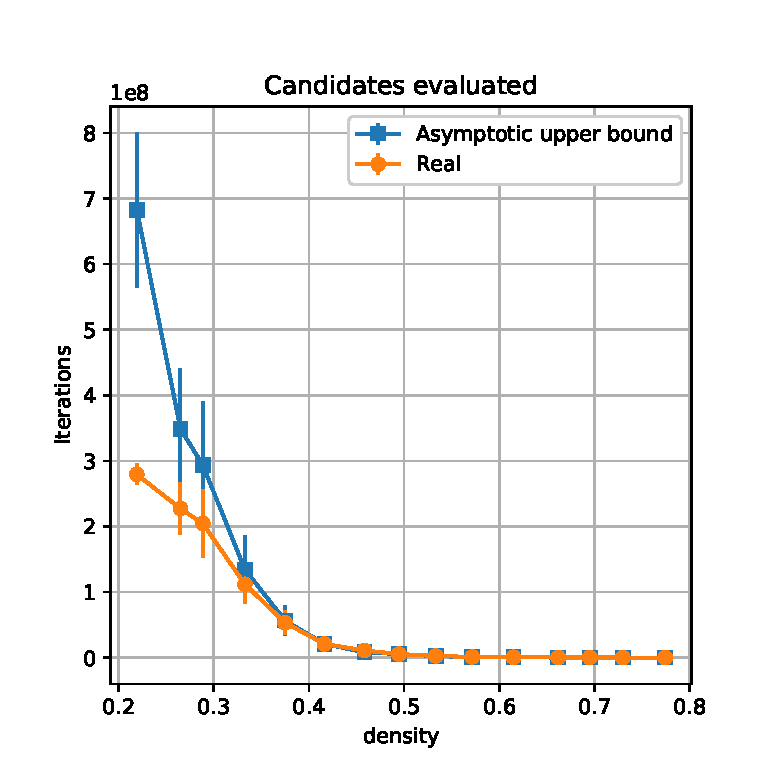
\includegraphics[height=2.5in]{Candidates_vs_SearchSpace.eps}
			\end{center}
			\caption{Evaluated candidates and search space as a function of the density.}\label{fig:candidates}
		\end{minipage}
	\end{figure}
	
	Figure~\ref{fig:info_vs_noInfo} shows the average runtime for MinReduct with and without knowing a priori the value of $k$, as a function of the density of 1's in the synthetic basic matrices. The 500 matrices were divided into 15 bins by discretizing the range of densities, for clarity purposes. The vertical bars show the standard deviation of each bin. Although in all cases the number of candidates evaluated when the value of $k$ is provided at the beginning of the algorithm is lower, there is no significant runtime reduction, as it can be seen in Figure~\ref{fig:info_vs_noInfo}. 
	
	In order to validate Equation~\ref{eq:ss2} for these synthetic matrices, we show in Figure~\ref{fig:candidates} the real number of evaluated candidates and the asymptotic upper bound computed by Equation~\ref{eq:ss2}. The real number of evaluated candidates is lower in most cases because of the pruned combinations.
	
	In MinReduct, the time complexity for the evaluation of combinations that do not include the last column of the arranged basic matrix ($c_{max}$) is $\Theta(m)$. The worst case time complexity for those combinations including $c_{max}$ is $\Theta(nm)$, because the exclusion evaluation may be required. The number of such combinations ($ss_{c_{max}}$) has an asymptotic upper bound as shown in Equation~\ref{eq:c_max2}.
	
	\begin{equation*}
	ss_{c_{max}}= O\left(\frac{1}{n-1}\sum_{i=1}^{k} \binom{n}{i} - \frac{1}{n_0-1}\sum_{i=1}^{\mathrm{min}(n_0,k)} \binom{n_0}{i}\right)\label{eq:c_max1}
	\end{equation*}
	\begin{equation}
	ss_{c_{max}}= O\left(\frac{1}{n}\sum_{i=1}^{k} \binom{n}{i} - \frac{1}{n_0}\sum_{i=1}^{\mathrm{min}(n_0,k)} \binom{n_0}{i}\right)\label{eq:c_max2}
	\end{equation}
	
	Thus, we can compute the upper bound of the asymptotic time complexity ($T_{MR}$) for MinReduct by the following expression:
	
	\begin{equation}
	T_{MR} = O\left(m*ss + mn*ss_{c_{max}}\label{eq:T1}\right)
	\end{equation}
	
	\begin{equation*}
	T_{MR} = O\left(m\left[\sum_{i=1}^{k} \binom{n}{i} - \sum_{i=1}^{\mathrm{min}(n_0,k)} \binom{n_0}{i}\right]+mn\left[\frac{1}{n}\sum_{i=1}^{k} \binom{n}{i} - \frac{1}{n_0}\sum_{i=1}^{\mathrm{min}(n_0,k)} \binom{n_0}{i}\right]\right)
	\end{equation*}	
	
	\begin{equation}
	T_{MR} = O\left(m\left[2\sum_{i=1}^{k} \binom{n}{i} - \left(1 + \frac{n}{n_0}\right)\sum_{i=1}^{\mathrm{min}(n_0,k)} \binom{n_0}{i}\right]\right)\label{eq:T2}
	\end{equation}	
	
%	Space complexity of MinReduct consist of two main components: the space required for storing the set of all the shortest reducts, and the space required for the candidate evaluation. The number of elements in set of all the shortest reducts is exponentially related to $n$. The space required for candidate evaluation in MinReduct is $\Theta(mn)$ because of the evaluations are performed in--place.
	
%
\section{Experimental comparison}\label{Comparison}
%	
	In this section, an experimental comparison of MiLIT and MinReduct is presented. For this purpose, the 500 synthetic matrices described above are used. In addition, the algorithms will be tested over 13 decision systems taken from the UCI machine learning repository~\cite{Bache13} and 15 high dimension synthetic basic matrices. All experiments were run on a PC with a Core i3-7100 Intel processor at 3.90GHz, with 8GB in RAM, running GNU/Linux. The source code of the algorithms, as well as all datasets and synthetic basic matrices used in our experiments, can be downloaded from \url{http://ccc.inaoep.mx/~ariel/MRvsMiLIT}. We thankfully acknowledge the authors of MiLIT~\cite{Piza20} for sharing the source code of their Java implementations of the MiLIT algorithm. 	
	
	\begin{figure}[hbt] 
		\begin{minipage}[t]{.48\linewidth}
			\begin{center}
				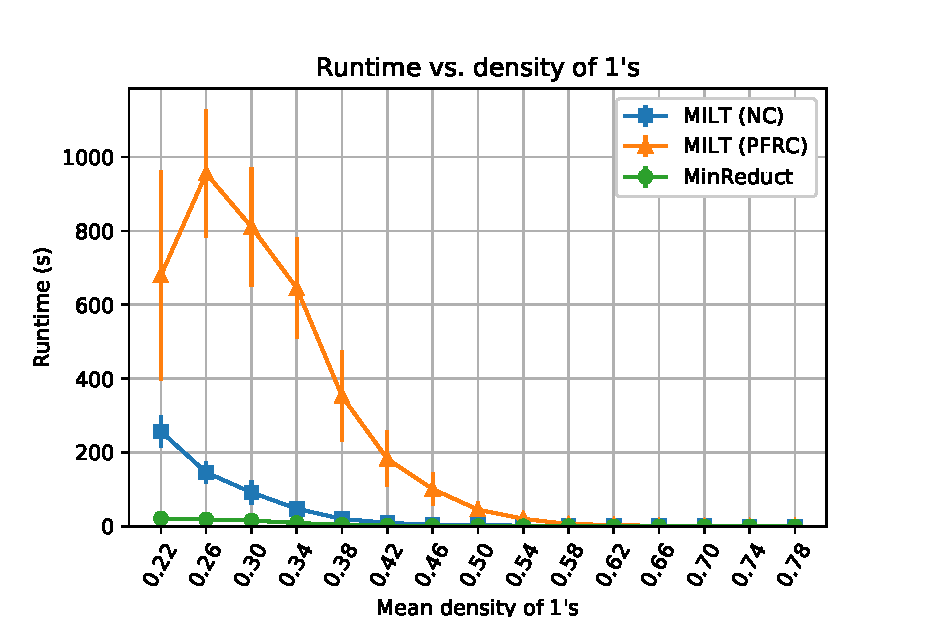
\includegraphics[height=2.5in]{MinReduct_vs_milt.eps} 
			\end{center}
			\caption{Average runtime vs. density of 1’s for MinReduct and MiLIT.}\label{fig:sinthyetic}
		\end{minipage}
		\begin{minipage}[t]{.48\linewidth}
		\begin{center}
			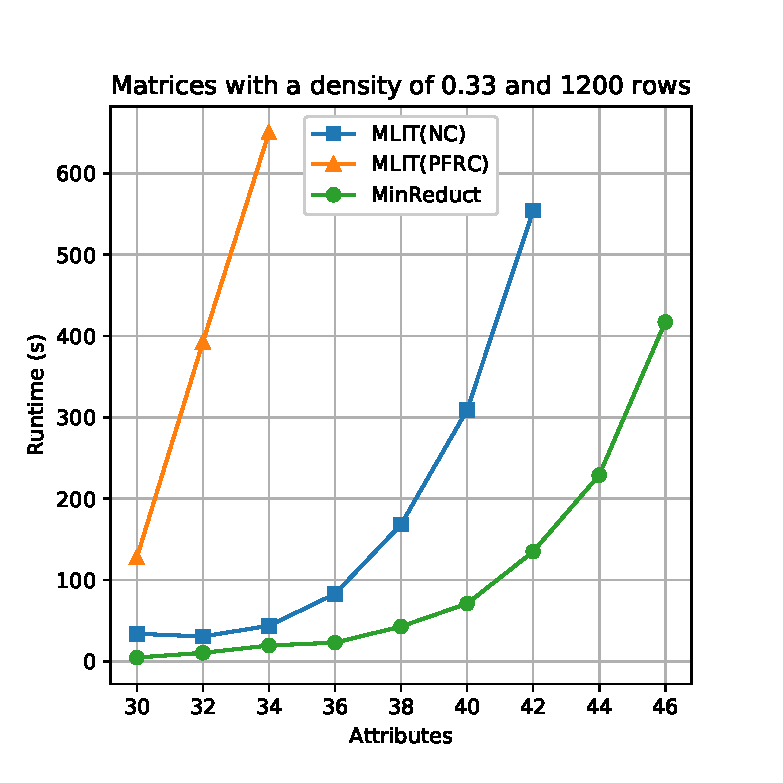
\includegraphics[height=2.5in]{low_density_Minreduct_vs_MLIT.eps} 
		\end{center}
		\caption{Runtime for matrices with 1200 rows and density 0.33.}\label{fig:1200x110}
		\end{minipage}
	\end{figure}		
	
	Figure~\ref{fig:sinthyetic} shows the average runtime for MiLIT (NC and PFRC) and MinReduct as a function of the density of 1’s over the 500 synthetic basic matrices described in the last section.  As it can be seen in Figure~\ref{fig:sinthyetic}, MinReduct was the fastest in general. 
	
	Figure~\ref{fig:1200x110} shows the runtime of MiLIT (NC and PFRC) and MinReduct for matrices with 1200 rows and density 0.33 with a number of columns ranging from 30 to 54. These matrices were included in order to explore the performance of the algorithms when the number of attributes increases. For these matrices MinReduct was also the fastest algorithm without any apparent relation to the number of attributes of the basic matrix.
	
	\begin{table}[htb]
		%\small
		\caption{Runtime over synthetic and real--world data.}
		\centering
		\begin{tabular}{lrrrrrccc}\label{tab:comparison}
			Name  & Atts& Objs & Dens & \multicolumn{1}{c}{Nsol} & Len & MR & NC & PFRC\\
			\hline			
			Keyword-activity & 37  & 1530 & 0.04 & 1      & 25 & 396 & 1111342 & \textbf{6}\\
			Soybean          & 35  & 307  & 0.11 & 29     & 11 & 283 & 23021 & \textbf{8}\\
			QSAR-biodeg      & 42  & 1055 & 0.12 & 2      & 13 & 264 & 254220 & \textbf{132}\\
			Anneal           & 38  & 63   & 0.21 & 15     & 7  & \textbf{18} & 135 & 50\\
			Dermatology      & 35  & 366  & 0.34 & 137    & 6  & \textbf{96} & 125 & 695\\
			Student-mat      & 32  & 395  & 0.43 & 21     & 6  & 174 & \textbf{159} & 27387\\
			Lung-cancer      & 57  & 32   & 0.47 & 112    & 4  & \textbf{25} & 56 & 81\\
			Arrhythmia       & 279 & 452  & 0.54 & 5      & 1  & \textbf{5} & 192 & 186\\
			Optdigits (train)& 64  & 382  & 0.59 & 185    & 4  & \textbf{278} & 1989 & 12986\\
			Landsat (test)   & 36  & 2000 & 0.74 & 6      & 14 & \textbf{1.6E6} & $>$12.6E6 & $>$12.6E6\\
			1500x150 		 & 150 & 1500 & 0.75 & 228778 & 4  & \textbf{2286} & 21998 & 37855 \\
			250x600 		 & 600 & 250  & 0.84 & 170    & 2  & 269 & \textbf{104} & 127 \\
			SPECT Heart      & 22  & 267  & 0.90 & 17     & 3  & $\mathbf{<1}$ & 2 & 1\\
			Ozone            & 72  & 575  & 0.93 & 239    & 2  & \textbf{7} & 87 & 141\\
			Sonar            & 60  & 208  & 0.95 & 2612   & 4  & \textbf{191} & 1607 & 4843\\
		\end{tabular}             
	\end{table}  
	
	Table~\ref{tab:comparison} shows the runtime of MiLIT (NC and PFRC) and MinReduct (MR), in milliseconds, for 13 decision systems taken from the UCI machine learning repository and two high dimensions synthetic basic matrices. This is a more heterogeneous experiment in terms of density and dimensions than our two previous experiments. The first columns in Table~\ref{tab:comparison} shows the name of the dataset, the number of attributes (Atts), the number of objects (Objs), the density of the basic matrix (Dens), the number of shortest reducts (Nsol) and the length of the  shortest reducts (Len). Decision systems in Table~\ref{tab:comparison} are sorted in ascending order of the density of their basic matrix. Although MinReduct was the fastest in most cases, for the first three matrices, PFRC--MiLIT showed a significant runtime reduction regarding MinReduct and NC--MiLIT. This result corresponds to the benefits expected from the application of Proposition~\ref{prop:zrPrevail} for sparse matrices.
%
\subsection{Discussion}
%	
	As a result of these experiments carried out over 528 matrices,  NC--MiLIT was the fastest algorithm in 11 matrices with no significant runtime reduction in any case. On the contrary, PFRC--MiLIT was the fastest algorithm in only three matrices, but it showed a significant runtime reduction in those matrices.  
	
	PFRC--MiLIT incorporates pruning strategies over the feature power set to make fewer evaluations than NC--MiLIT. However, using a breadth--first search for finding all the shortest reducts, although guarantees that no combination with length higher than $k$ is evaluated, is less efficient in terms of time and space, than the traditional depth--first search used in most algorithms for reduct computation. As it was shown in Figure~\ref{fig:info_vs_noInfo}, there is no significant advantage in having such restriction of the search space in MinReduct. Thus, from our experiments we conclude that the evaluation of Proposition~\ref{prop:zrPrevail} for sparse matrices is the main contribution of PFRC--MiLIT. In~\cite{Piza20} an upper threshold density of 0.3 was estimated for the application of  PFRC--MiLIT. After our experiments, we recommend to reduce this value to 0.15.   	
	
	\begin{figure}[hbt] 
		\begin{minipage}[t]{.48\linewidth}
			\begin{center}
				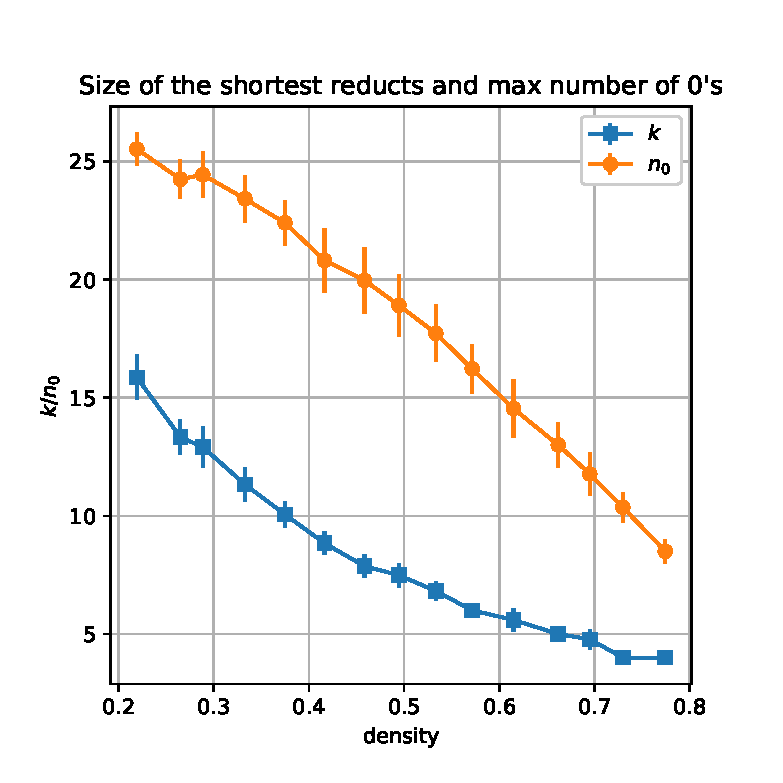
\includegraphics[height=2.5in]{Length_and_N0_vs_denisty.eps} 
			\end{center}
			\caption{Behavior of $k$ and $n_0$ as a function of the density of the basic matrix.}\label{fig:n0}
		\end{minipage}
		\begin{minipage}[t]{.48\linewidth}
			\begin{center}
				\includegraphics[height=2.5in]{fraction.eps} 
			\end{center}
			\caption{Behavior of $k/2$ and the fraction of the runtime of NC--MiLIT and MinReduct.}\label{fig:fraction}			
		\end{minipage}
	\end{figure} 
	
	Figure~\ref{fig:n0} shows the behavior of $k$ and $n_0$ as a function of the density for the 500 synthetic matrices used in our first experiment. This behavior, together with Equation~\ref{eq:T2}, explain the reason for the relatively low cost of computing reducts in matrices with a high density of ones.
	
	NC--MiLIT evaluates all the combinations in the search space defined by Equation~\ref{eq:ss2}, without using any pruning property. From the asymptotic complexity point of view, MinReduct (Equation~\ref{eq:T2}) is at least $k/2$ faster than NC--MiLIT (Equation~\ref{eq:complexNC}). This relation between the runtime of MinReduct and NC--MiLIT can be experimentally corroborated taking the values of $k$ from Figure~\ref{fig:n0} and the runtimes shown in Figure~\ref{fig:sinthyetic}. For this purpose, in Figure~\ref{fig:fraction} we show the value of $k/2$ and the fraction of the runtime of NC--MiLIT over MinReduct as a function of the density of 1's. Thus, we can conclude that using MinReduct instead of NC--MiLIT is a better option in general.

	
%
\section{Conclusions} \label{conclusions}
%	
	In this paper we present a comparative study of MiLIT and MinReduct: two recent algorithms for computing all the shortest reducts (minimum length irreducible testors). Although MiLIT comes from the Testor Theory and MinReduct comes from the Rough Set Theory, both algorithms are intended to solve an equivalent algorithmic task. A description of the algorithms in terms of asymptotic complexity was presented. Finally, an experimental comparison over synthetic basic matrices and real--world decision systems taken from the UCI machine learning repository was carried out. 
	
	From our experiments, we have concluded that PFRC--MiLIT is the fastest algorithm for spare basic matrices with densities under 0.15. The main advantage of PFRC--MiLIT relays on the evaluation of the zero row prevalence on these spare matrices. We have also found that the breadth--first search used in MiLIT is less efficient than the traditional depth--first search used in MinReduct, for candidate evaluation. Thus, MinReduct was faster than MiLIT for basic matrices with densities above 0.15 in most cases.
	
	An interesting study for future work would be assessing the performance of verifying the zero row prevalence using a depth--first search, for spare basic matrices.
 
% ---- Bibliography ----
%
\bibliography{mybib}{}
\bibliographystyle{splncs03}

\end{document}
